\documentclass[a4paper,10pt,oneside]{jsbook}
%
\usepackage{amsmath,amssymb,bm}
\usepackage{bm}
\usepackage[dvipdfmx]{graphicx}
\usepackage{ascmac}
\usepackage{makeidx}
\usepackage{txfonts}
\usepackage{indentfirst}
\usepackage{booktabs}
\usepackage{tabularx}
\usepackage{comment}
\AtBeginDvi{\special {pdf:tounicode EUC-UCS2}}
\usepackage[dvipdfmx, setpagesize=false, bookmarks=true, bookmarksnumbered=true]{hyperref}
\usepackage{nameref}
\usepackage{url}
%
\makeindex
%
\newcommand{\diff}{\mathrm{d}}            %微分記号
\newcommand{\divergence}{\mathrm{div}\,}  %ダイバージェンス
\newcommand{\grad}{\mathrm{grad}\,}       %グラディエント
\newcommand{\rot}{\mathrm{rot}\,}         %ローテーション
%
\setlength{\textwidth}{\fullwidth}
\setlength{\textheight}{44\baselineskip}
\addtolength{\textheight}{\topskip}
\setlength{\voffset}{-0.6in}
%

\begin{document}

%%%%%%%%%%%%%%%%%%%%%%%%%%%%%%%%%%%%%%%%%%%%%%%%%%%%%
% 表紙
\begin{titlepage}
\noindent
国立大学法人 東京大学 生産技術研究所 御中
\begin{center}
	\vspace{8cm}
	{\Huge \textbf{HPC/PFポータルGUI操作説明書}} \\
	\vspace{10cm}
	{\Large \textbf{2015年3月20日}} \\
	\vspace{0.5cm}
	{\Large \textbf{株式会社イマジカデジタルスケープ}}
\end{center}
\end{titlepage}

%%%%%%%%%%%%%%%%%%%%%%%%%%%%%%%%%%%%%%%%%%%%%%%%%%%%%
% 目次
\tableofcontents

%%%%%%%%%%%%%%%%%%%%%%%%%%%%%%%%%%%%%%%%%%%%%%%%%%%%%
% 本文
%%%%%%%%%%%%%%%%%%%%%%%%%%%%%%%%%%%%%%%%%%%%%%%%%%%%%
\chapter{はじめに}
本書ではHPC/PFポータルGUIの操作方法について解説します.

\section{動作環境とインストール}
ポータルGUIは以下の環境で動作します.
\begin{tabbing}
0123\=01234567890123\=0123456789\kill
\> OS \> : Linux, Windows(Vista,7,8), MacOSX \\
\> Webブラウザ \> : Mozilla Firefox 15.x, Google Chrome 21.x, Apple Safari 6.x, Windows Internet Explorer 10.x 
\end{tabbing}

\section{ポータルGUIのインストール}

\subsection{Node.jsのインストール}
ポータルGUIの動作にはNode.jsのインストールが必要です.\\
Node.jsの公式サイト(\verb+http://nodejs.org/+)からNode.js本体をダウンロードし,インストールします.

\subsection{SSHクライアントのインストール}
ポータルGUIを使ったリモートジョブの実行にはSSHクライアントのインストールが必要です.\\
WindowsでのポータルGUIの動作にはOpenSSH for Windowsを用います.\\
以下のリンクなどからOpenSSH for Windowsをダウンロードし,SSHクライアントをインストールします.\\
(サーバーのインストールは不要です) \\
    \url{http://www.mls-software.com/opensshd.html}

\subsection{ポータルGUIアプリケーションの準備}
ポータルGUIアプリケーションの最新版をgithubからダウンロードします.
\begin{verbatim}
   $git clone https://github.com/avr-aics-riken/hpcpfGUI.git
\end{verbatim}
もしくは以下のリンクからzipファイルをダウンロードし,展開します.\\
	\url{https://github.com/avr-aics-riken/hpcpfGUI/archive/master.zip}

\newpage

\subsection{Node.jsサブモジュールのインストール}
ポータルGUIアプリケーションを展開したディレクトリに,
ポータルGUIで利用しているNode.jsの必要なサードパーティモジュールのインストールを行います.
\begin{verbatim}
   $cd bin
   $sh install.sh 
   (Windows版は install.bat)
\end{verbatim}

\newpage

\subsection{設定ファイルの編集}
\label{sec:editconfig}
ポータルGUIの基本設定を行います.\\
ポータルGUIを展開したディレクトリ下のconf/hpcpfGUI.conf
を書き換える事で設定を行います.\\

\subsubsection{設定ファイルの書式}
設定ファイルの書式は以下の通りです.
\label{sec:editconfig_format}
\begin{tabbing}
0123\=0123456789012345678\=0123456789\=0123456789\kill
\> "port"     \>:\ \ サーバーの使用するポートを指定します(デフォルト:8080)\\
\> "アプリ名(例:PDI)" \>:\ \ アプリケーションのボタン上での表示名を指定します\\
\>                 \>"win32" \>:\ \ Windowsでの起動コマンドを指定します\\
\>                 \>"darwin" \>:\ \ OSXでの起動コマンドを指定します\\
\>                 \>"linux" \>:\ \ Linuxでの起動コマンドを指定します\\
\>                 \>"extension" \>:\ \ アプリケーションに対応付けるファイル拡張子を\\
\>                 \>                    \>\  \ セミコロン区切りで指定します.(例: ".pdi")\\
\end{tabbing}

\  \ 設定ファイルにツールを追加する場合の記述例は以下の通りです.
\begin{tabbing}
0123\=0123456789012345678\=0123456789\=0123456789\kill
\> "Emacs" : \{ \\
\> \> "win32"    : "$\backslash$"C:$\backslash$$\backslash$Program Files$\backslash$$\backslash$Emacs$\backslash$$\backslash$emacs.exe$\backslash$"",\\
\> \> "darwin" : "/Applications/Emacs.app/Contents/MacOS/Emacs",\\
\> \> "linux"  : "emacs",\\
\> \> "extension" : ".obj;.txt"\\
\> \}\\
\end{tabbing}

ツール設定を追加すると, プロジェクト編集画面で,拡張子に対応したファイルを選択すると,ツール起動ボタンが表示されます. プロジェクト編集画面の操作詳細は第\ref{chap:projeditor}章 \nameref{chap:projeditor}をご参照下さい.

\newpage
\section{ポータルGUIの起動}
起動スクリプトを実行するとポータルGUIサーバーが起動します.
\begin{verbatim}
   $sh run_hpcpfGUI.sh
   (Windows版は run_hpcpfGUI.bat)
\end{verbatim}

\section{ポータルGUIへのアクセス}
ポータルGUIは,Webブラウザのアドレス欄に「http://localhost:8080」と入力することでアクセス出来ます.\\
(ポートは設定ファイルで編集する事が出来ます. セクション \ref{sec:editconfig} をご覧下さい.)

\chapter{ホーム画面}
ホーム画面では,以下の操作を行う事が出来ます.
\begin{itemize}
	\item 新規プロジェクト作成
	\item プロジェクトアーカイブを開く
	\item 既存プロジェクトを開く
	\item 最近開いたプロジェクトを開く
	\item リモートホストの登録
	\item ファイルブラウザを開く
	\item Knowledge DBへのアクセス
\end{itemize}

\begin{figure}[htbp]
	\begin{center}
		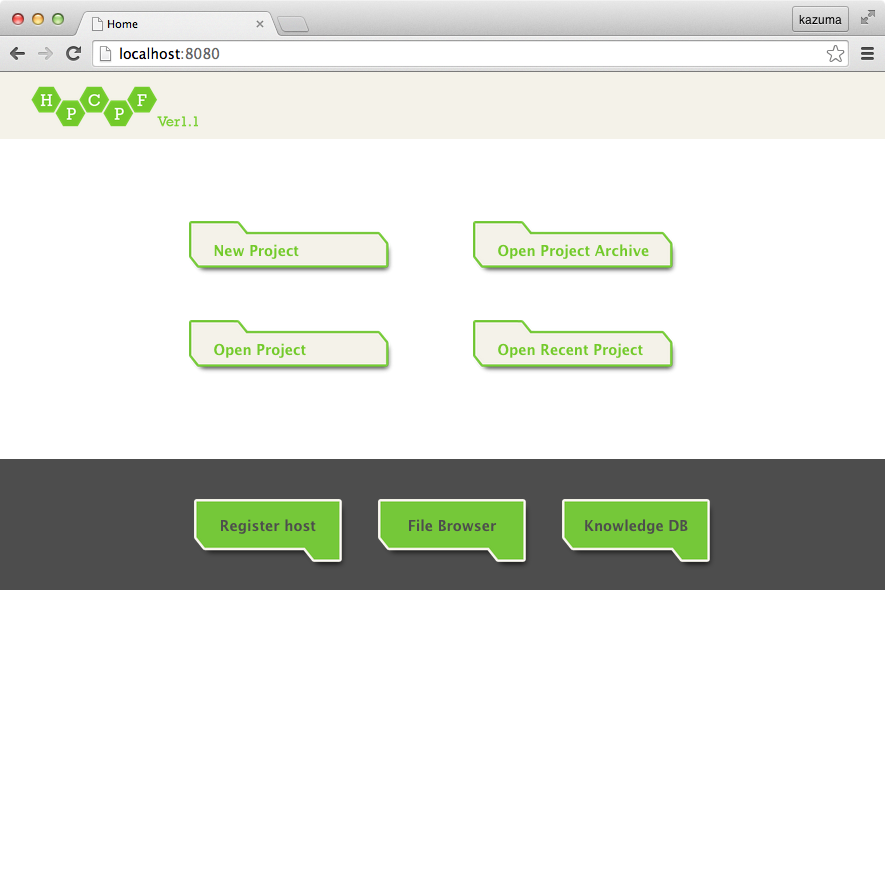
\includegraphics[width=11.5cm]{image/home_000.png}
	\end{center}
	\caption{ホーム画面}
	\label{fig:home}
\end{figure}


\section{新規プロジェクト作成}
「New Project」ボタンを押しプロジェクト名を入力することで,新規プロジェクトが作成されます.\\
(※制限事項: プロジェクト名やファイル/フォルダ名には日本語名は使用できません)

\section{既存プロジェクトを開く}
以下の操作で既存のプロジェクトを開く事が出来ます.
\begin{enumerate}
	\item 「OpenProject」ボタン(図\ref{fig:home}左下)を押すとファイルダイアログ(図\ref{fig:home_dialog})が開きます
	\item ダイアログ上で開きたいプロジェクトディレクトリを選択します
	\item 「Open」ボタンを押すとプロジェクトが開き,プロジェクト編集画面へと移動します\\
			プロジェクト編集画面の操作詳細は第\ref{chap:projeditor}章 \nameref{chap:projeditor}をご参照下さい
\end{enumerate}

\section{プロジェクトアーカイブを開く}
以下の操作でプロジェクトアーカイブを開くことが出来ます.
\begin{enumerate}
	\item 「OpenProjectArchive」ボタン(図\ref{fig:home}右上)を押すとファイルダイアログ(図\ref{fig:home_dialog})が開きます
	\item ダイアログ上で開きたいプロジェクトアーカイブ(.tar.gzファイル)を選択します
	\item 「Open」ボタンを押し, プロジェクトアーカイブの展開フォルダ名を入力します
	\item 「New」ボタンを押すとプロジェクトアーカイブが展開され,プロジェクト編集画面へと移動します\\
			プロジェクト編集画面の操作詳細は第\ref{chap:projeditor}章 \nameref{chap:projeditor}をご参照下さい
\end{enumerate}

\begin{figure}[htbp]
	\begin{center}

		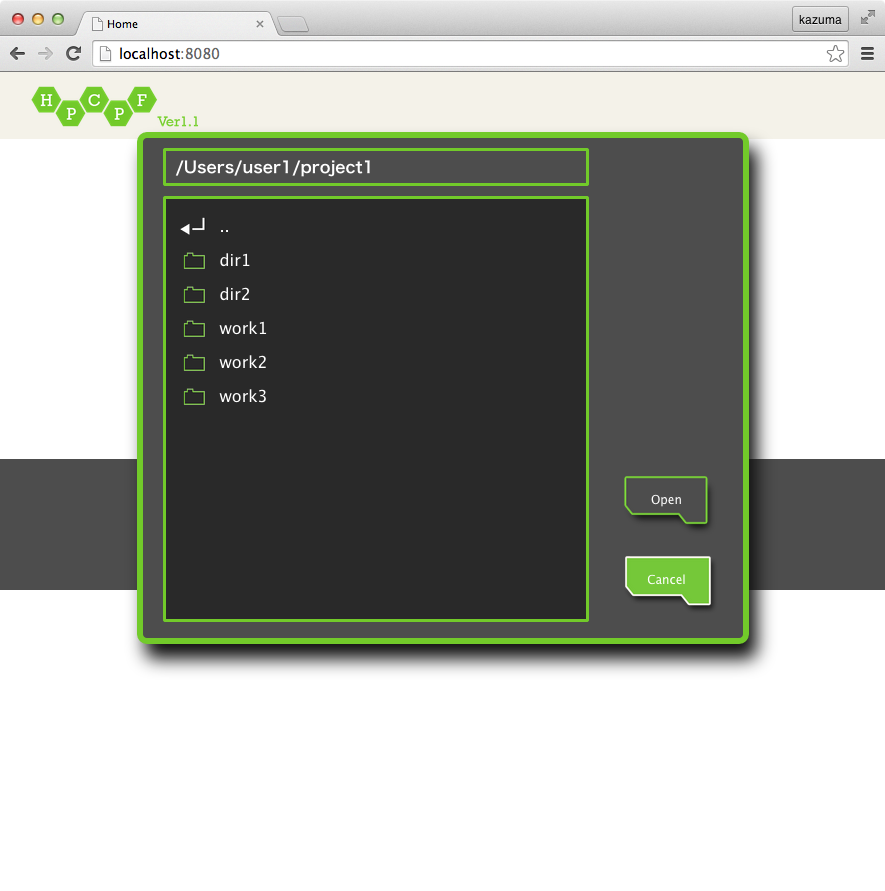
\includegraphics[width=11cm]{image/home_001.png}
	\end{center}
	\caption{ファイルダイアログ}
	\label{fig:home_dialog}
\end{figure}

\newpage 

\section{最近開いたプロジェクトを開く}
「Recent Project」枠内に最近開いたプロジェクトが表示されます.その中からプロジェクトを選択すると,そのプロジェクトを開く事が出来ます.
プロジェクト編集画面の操作詳細は第\ref{chap:projeditor}章 \nameref{chap:projeditor}をご参照下さい.

\section{リモートホスト登録}
「Register Remote host」ボタンを押すと,リモートホスト登録画面が開きます.
リモートホスト登録画面の操作詳細は第\ref{chap:remotehost}章 \nameref{chap:remotehost}をご参照下さい.

\section{ファイルブラウザ}
「File Browser」ボタンを押すと,ファイルブラウザ画面が開きます.
ファイルブラウザ画面の操作詳細は第\ref{chap:filebrowser}章 \nameref{chap:filebrowser}をご参照下さい.

\section{Knowledge DB}
「Knowledge DB」ボタンを押すと,知識データベースWebサイトが開きます.


\chapter{リモートホスト登録画面}
\label{chap:remotehost}
リモートホスト登録画面では,GUIポータルで使用するリモートホストのログイン情報を事前に登録します.

\begin{figure}[htbp]
	\begin{center}
		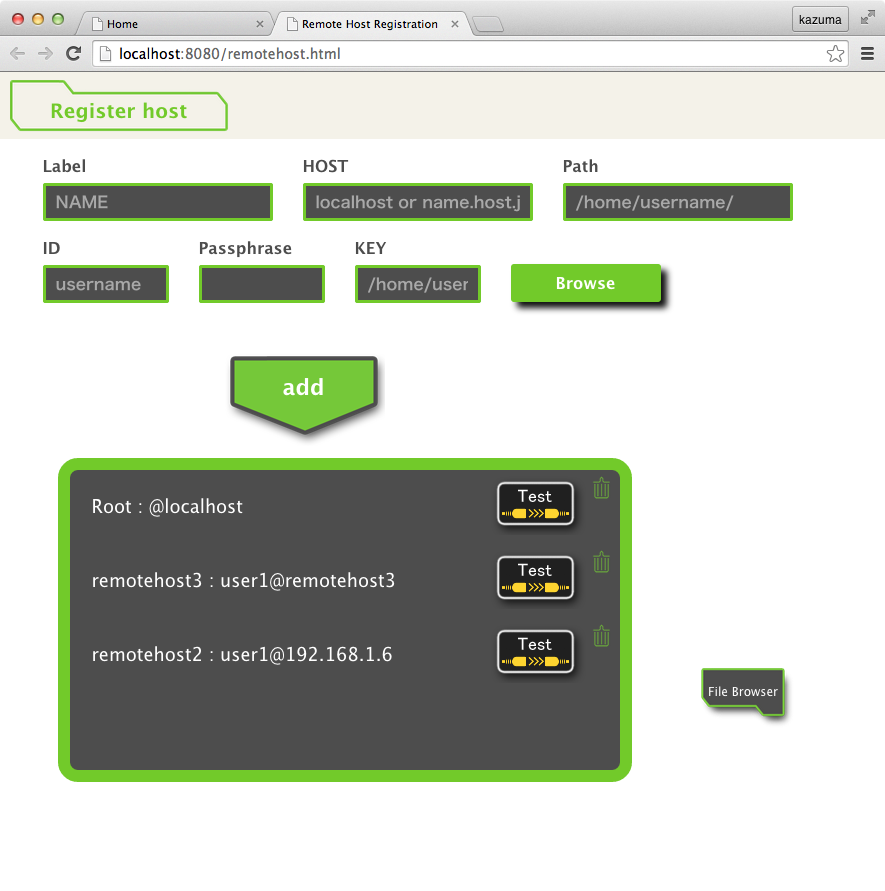
\includegraphics[width=12.0cm]{image/remotehost_000.png}
	\end{center}
	\caption{リモートホスト登録画面}
	\label{fig:remotehost}
\end{figure}

\newpage 

\section{リモートホストを登録する}
図\ref{fig:remotehost}の画面上部に必要な情報を入力します.
\begin{tabbing}
0123\=01234567890123\=0123456789\kill
\>「Label」\>:\ \ 登録名(ファイルブラウザでの表示名)\\
\>「HOST」\>:\ \ リモートホストのアドレス\\
\>「Path」\>:\ \ ログイン直後に開くディレクトリパス\\
\>「ID」\>:\ \ ログインID\\
\>「Password」\>:\ \ ログイン鍵のパスワード\\
\>「KEY」\>:\ \ ログイン鍵のファイルパス\\
\>「Browse」\>:\ \ ボタンを押すとファイルダイアログが開き,鍵ファイルを選択する事が出来ます
\end{tabbing}

以上を入力後,「add」ボタンを押すと,リモートホストが登録され,ホスト一覧に追加されます.
追加したホストはファイルブラウザにて使用することが出来ます.
ホスト一覧から登録済みのホストを選択すると,その設定(Passwordを除く)を入力欄にセットすることが出来ます.
また,入力欄のLabelと同一のLabelが既にホスト一覧に登録されている場合,「add」を押すと,既存の設定が上書きされます.

「File Browser」ボタン(図\ref{fig:remotehost}右下)を押すとファイルブラウザ画面が開きます. \\
ファイルブラウザ画面の操作詳細は第\ref{chap:filebrowser}章 \nameref{chap:filebrowser}をご参照下さい.

\newpage
\section{接続テスト}
登録したホストへの接続を事前にテストします.

\begin{figure}[htbp]
	\begin{center}
		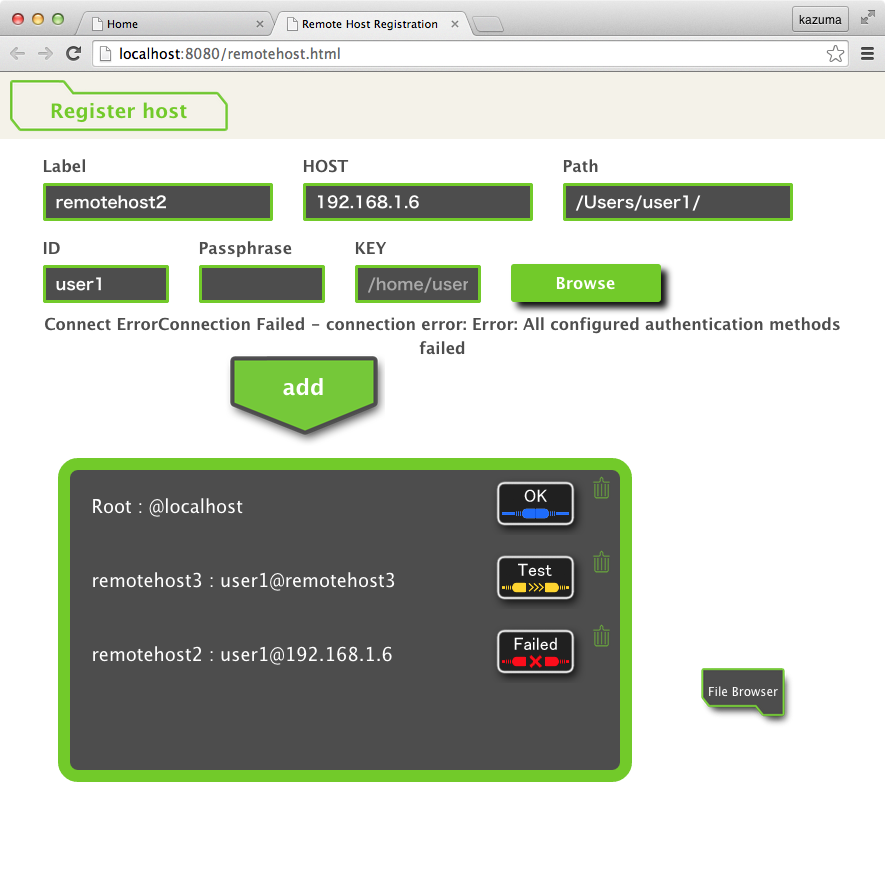
\includegraphics[width=12.0cm]{image/remotehost_001.png}
	\end{center}
	\caption{接続テスト}
	\label{fig:remotetest}
\end{figure}

ホスト一覧で,接続テストしたいホストの欄の右にある「Test」ボタンを押すと,接続テストが行われます.
接続が成功した場合「OK」,接続が失敗した場合「Fail」が表示されます.
「Fail」の場合,「Browse」ボタンの下にエラー内容が表示されます.
(図\ref{fig:remotetest})

\newpage
		
\section{リモートホストを登録解除する}
登録したホストを一覧から削除します.

\begin{figure}[htbp]
	\begin{center}
		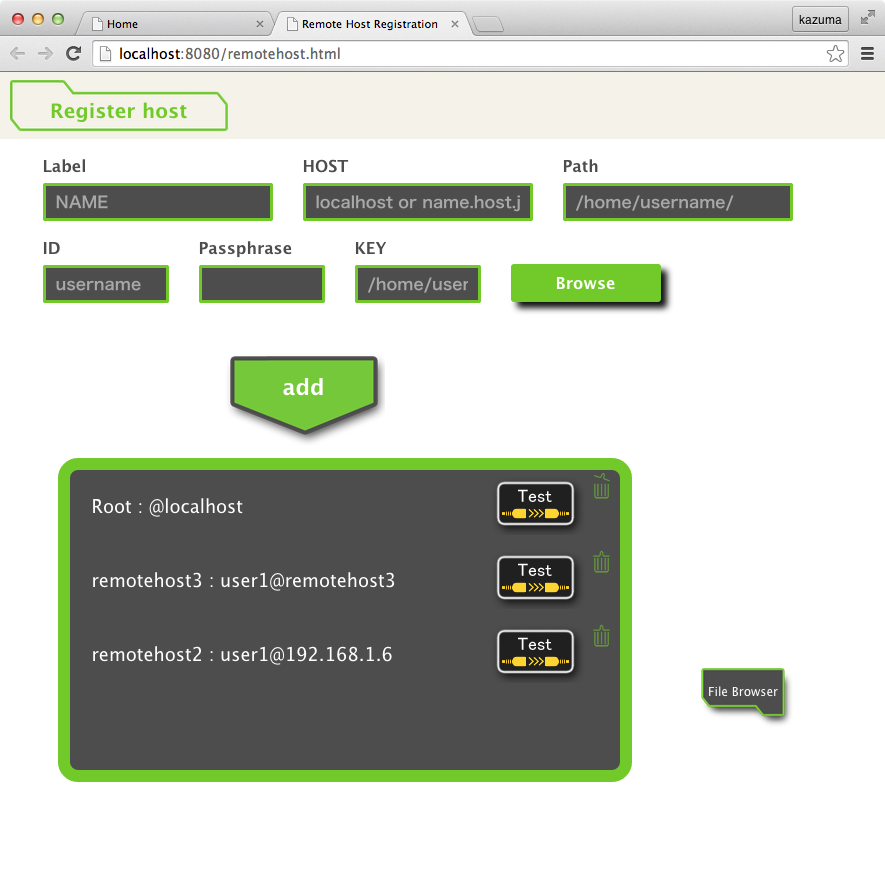
\includegraphics[width=12.0cm]{image/remotehost_002.png}
	\end{center}
	\caption{ホストの登録解除(蓋の開いた状態のアイコン)}
	\label{fig:remotedelete}
\end{figure}


ホスト一覧上で,削除したいホストの欄の右端にあるゴミ箱ボタンを押します.
ゴミ箱ボタンの絵が蓋の開いたアイコンへと変わります.再度ボタンを押すと,リモートホストが登録解除され,ホスト一覧から削除されます.
(図\ref{fig:remotedelete})


\chapter{ファイルブラウザ画面} 
\label{chap:filebrowser}
ファイルブラウザ画面では,ファイルのコピー,移動,削除,解凍,圧縮,リモートホストとのファイル転送を行います.

\begin{figure}[htbp]
	\begin{center}
		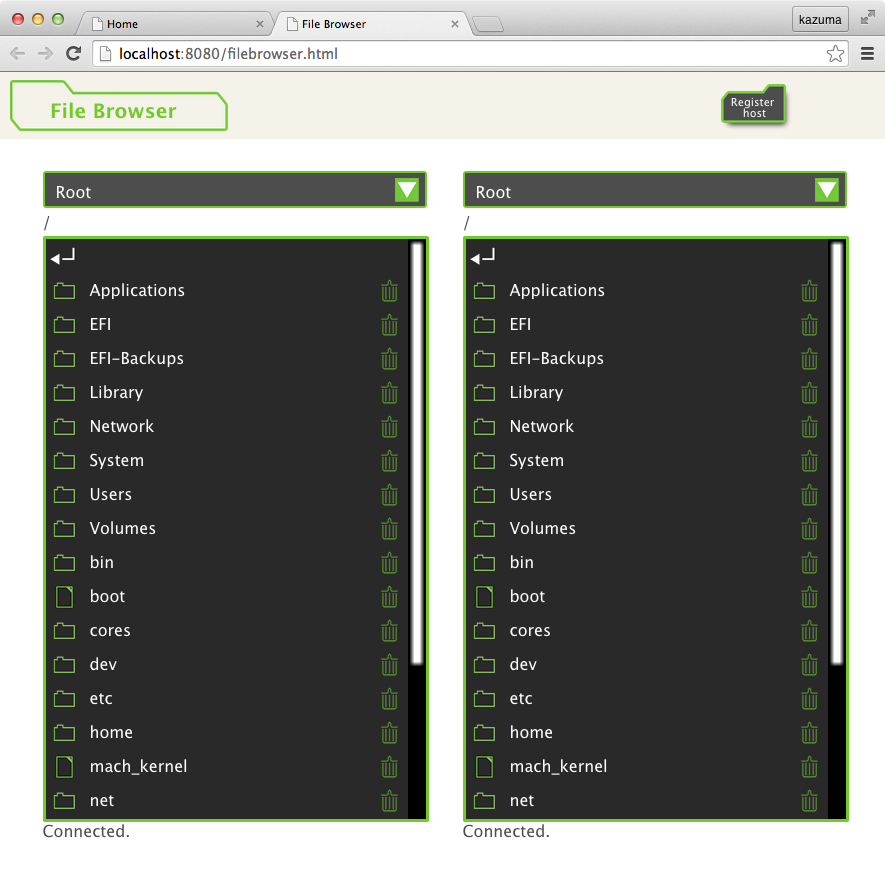
\includegraphics[width=12.0cm]{image/filebrowser_000.png}
	\end{center}
	\caption{ファイルブラウザ画面}
	\label{fig:filebrowser}
\end{figure}

\newpage



\section{共通操作}
\subsection{ホストの選択}
ファイルブラウザ画面では2つのペインを使用してファイルやディレクトリの操作を行います.\\
始めに,各ペインで表示・操作するホストを選択します.
各ペインのファイル一覧の上にあるプルダウンメニューから操作したいホストを選ぶと,
選択したホストのファイル一覧が表示されます(図\ref{fig:filebrowser_host}).

\begin{figure}[htbp]
	\begin{center}
		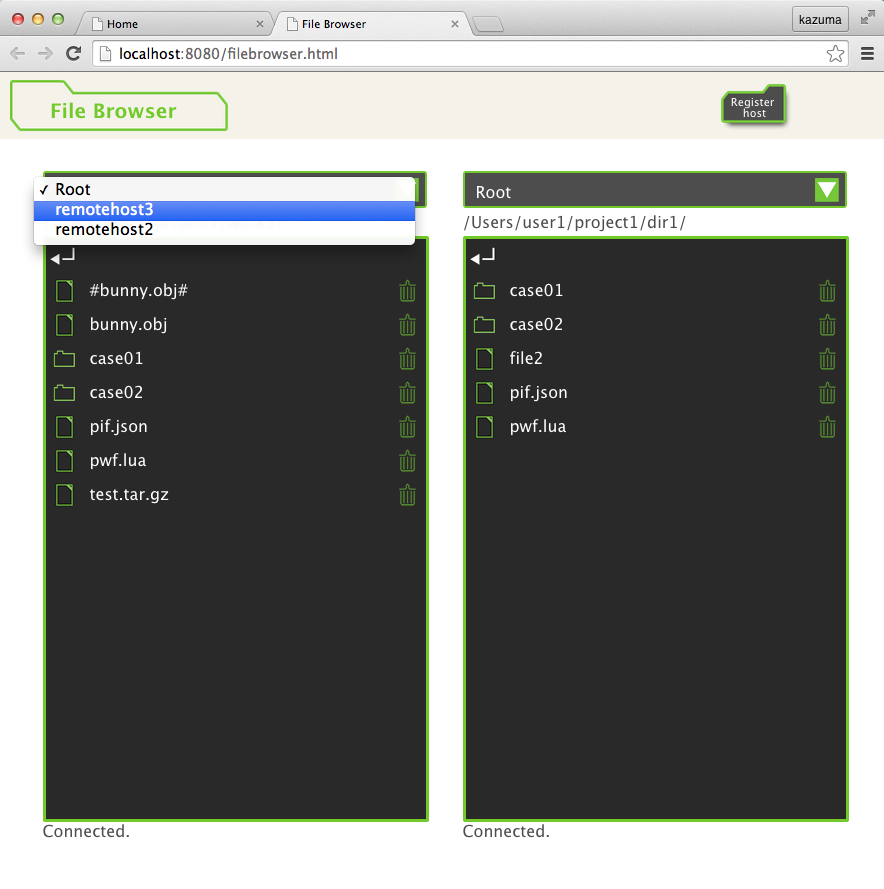
\includegraphics[width=12.0cm]{image/filebrowser_007.png}
	\end{center}
	\caption{ホストの選択}
	\label{fig:filebrowser_host}
\end{figure}


\subsection{ディレクトリ移動}
ファイル一覧の中からディレクトリを選択すると、ディレクトリ内のファイル一覧が表示されます.
上のディレクトリ階層に戻る場合,ファイル一覧の最上部にある「..」を押します.

\subsection{ファイルの削除}
\begin{enumerate}
	\item ファイル一覧上で,削除したいファイルの右にあるゴミ箱ボタンを押します.
	\item ゴミ箱ボタンの絵が蓋の開いたアイコンに変わります.
	\item 再度ゴミ箱ボタンを押すと,ファイルが削除されます.
\end{enumerate}

\section{ローカルホストの操作}
ローカルホスト内でのファイル操作を行うには,
両方のペインでホスト選択のプルダウンからローカルホストを選択しておきます.

\subsection{ファイルのコピー}
\begin{enumerate}
	\item 各ペインで,コピー元とコピー先のディレクトリを開きます.
	\item コピーしたいファイルもしくはディレクトリをコピー元のペインからドラッグしてコピー先のペインに重ねると,
		 ファイル操作メニューが表示されます.
	\item 「copy」上にドロップすることで,ドロップ先ディレクトリへのコピーが行われます.
\end{enumerate}
\begin{figure}[htbp]
	\begin{center}
		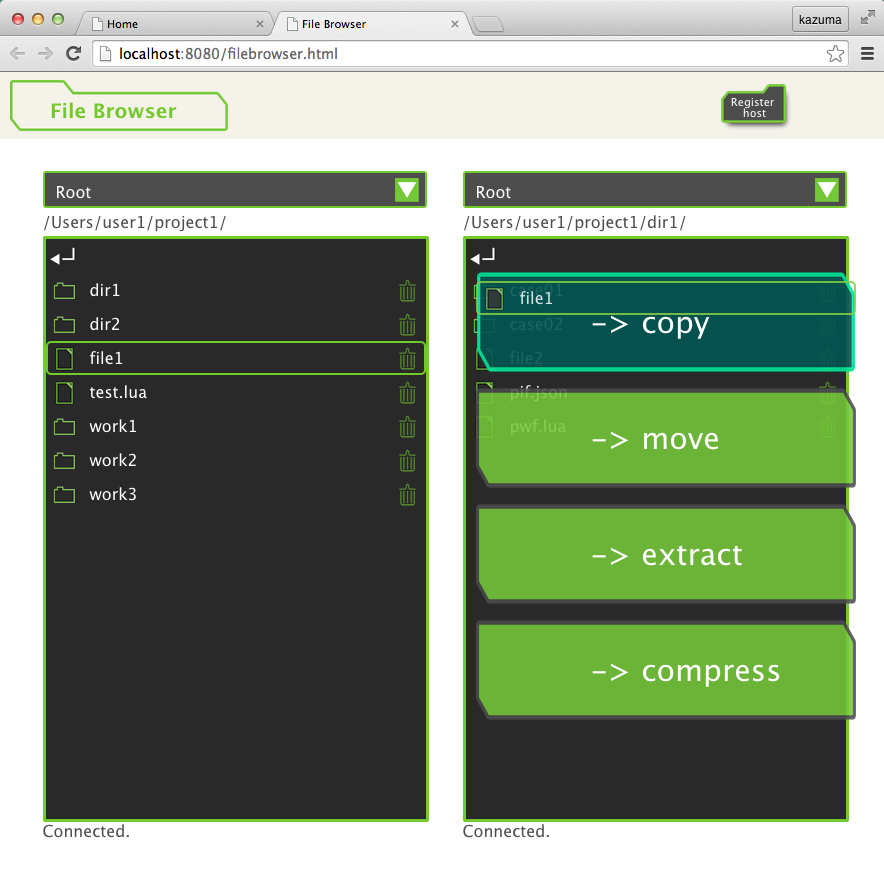
\includegraphics[width=12.0cm]{image/filebrowser_003.png}
	\end{center}
	\caption{ドラッグによるファイルのコピー}
	\label{fig:filebrowser_filecopy}
\end{figure}

\newpage

\subsection{ファイルの移動}
\begin{enumerate}
	\item 各ペインで,移動元と移動先のディレクトリを開きます.
	\item 移動したいファイルもしくはディレクトリを移動元のペインからドラッグして移動先のペインに重ねると,
		  ファイル操作メニューが表示されます.
	\item 「move」上にドロップすることで,ドロップ先ディレクトリへの移動が行われます.
\end{enumerate}
\begin{figure}[htbp]
	\begin{center}
		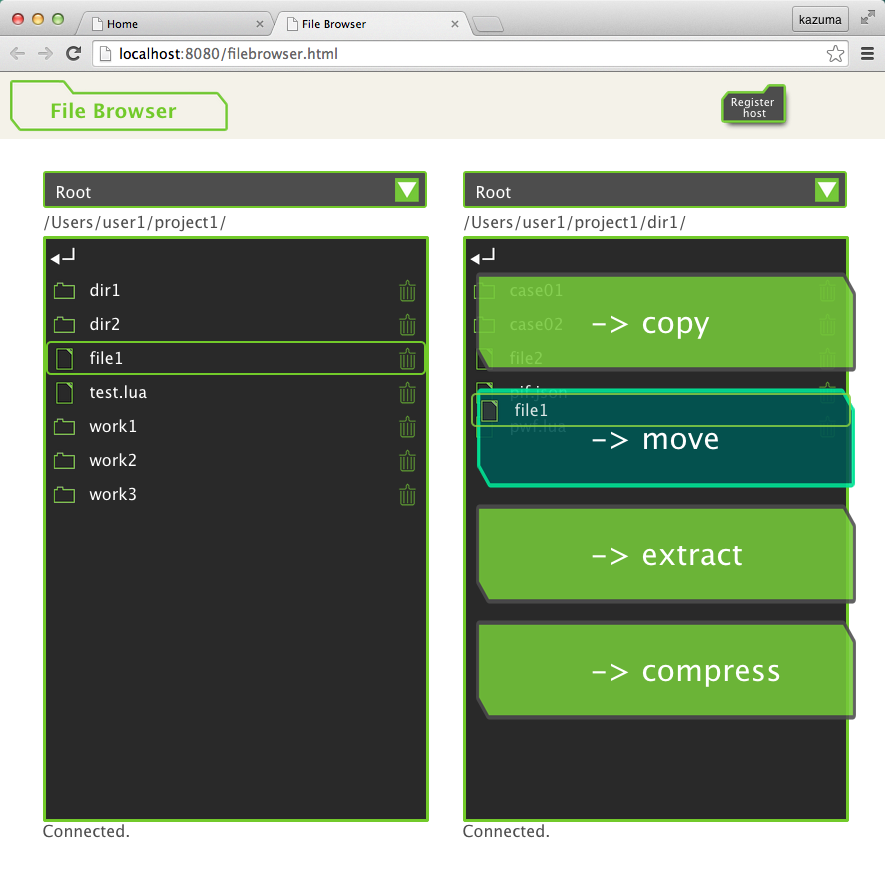
\includegraphics[width=12.0cm]{image/filebrowser_004.png}
	\end{center}
	\caption{ドラッグによるファイルの移動}
	\label{fig:filebrowser_filemove}
\end{figure}

\subsection{ファイル, ディレクトリ名の変更}
\begin{enumerate}
	\item 各ペインのファイル一覧で, ファイル名またはディレクトリ名を右クリックします.
	\item ポップアップ表示された入力ボックスに, 変更したいファイル名またはディレクトリ名を入力します.
	\item エンターキーを押すことで, ファイル名またはディレクトリ名が変更されます.
\end{enumerate}

\newpage

\subsection{ファイルの解凍}
\begin{enumerate}
	\item 各ペインで,圧縮ファイルの含まれるディレクトリと解凍先のディレクトリを開きます.
	\item 解凍したいファイルをドラッグして解凍先のペインに重ねると,ファイル操作メニューが表示されます.
	\item 「extract」上にファイルをドロップすることで,ファイルがドロップ先のディレクトリに解凍されます.
\end{enumerate}

\begin{figure}[htbp]
	\begin{center}
		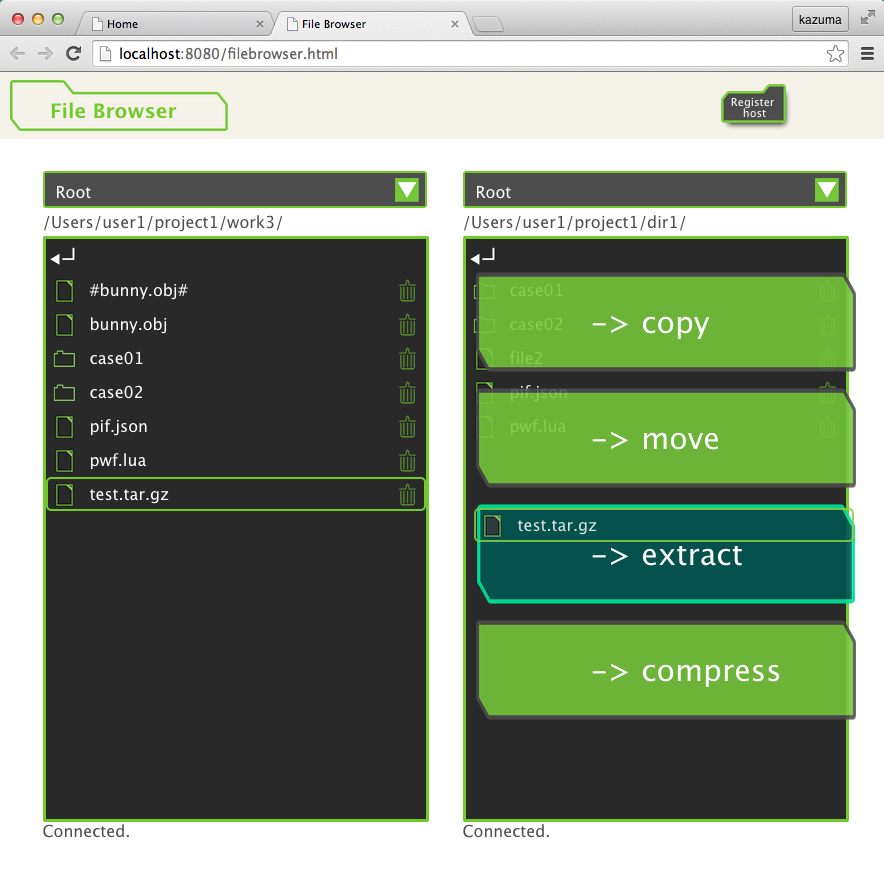
\includegraphics[width=12.0cm]{image/filebrowser_005.png}
	\end{center}
	\caption{ドラッグによるファイルの解凍}
	\label{fig:filebrowser_fileextract}
\end{figure}

\newpage

\subsection{ファイルの圧縮}
\begin{enumerate}
	\item 各ペインで,圧縮したいファイルもしくはディレクトリの含まれるディレクトリと圧縮先のディレクトリを開きます.
	\item 圧縮したいファイルもしくはディレクトリをドラッグして圧縮先のペインに重ねると,ファイル操作メニューが表示されます.
	\item「compress」上にドロップすることで,ドロップ先のディレクトリに圧縮されたファイルが生成されます.
\end{enumerate}

\begin{figure}[htbp]
	\begin{center}
		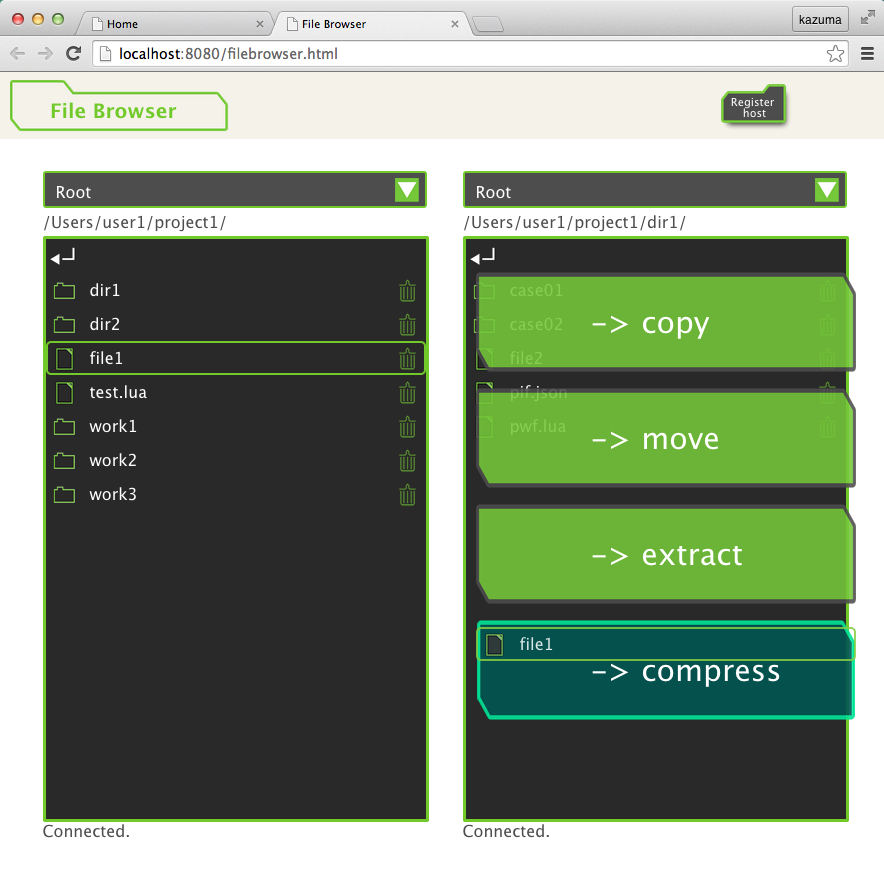
\includegraphics[width=12.0cm]{image/filebrowser_006.png}
	\end{center}
	\caption{ドラッグによるファイルの圧縮}
	\label{fig:filebrowser_filecompress}
\end{figure}

\newpage

\section{リモートホストの操作}
ローカルホストとリモートホスト間のファイル操作を行うには,
各ペインで,ホスト選択のプルダウンから操作対象のローカルホストとリモートホストを選択しておきます.
リモートホスト間ではファイルのアップロード,ダウンロードが可能です.
\subsection{ファイルのアップロード}
\begin{enumerate}
	\item 各ペインで,アップロード元(ローカルホスト)とアップロード先(リモートホスト)のディレクトリを開きます.
	\item アップロードしたいファイルもしくはディレクトリをアップロード元のペインからドラッグしてアップロード先のペインに重ねると,
		  ファイル操作メニューが表示されます.
	\item 「upload」上にドロップすることで,ドロップ先ディレクトリへのアップロードが行われます.
\end{enumerate}

\begin{figure}[htbp]
	\begin{center}
		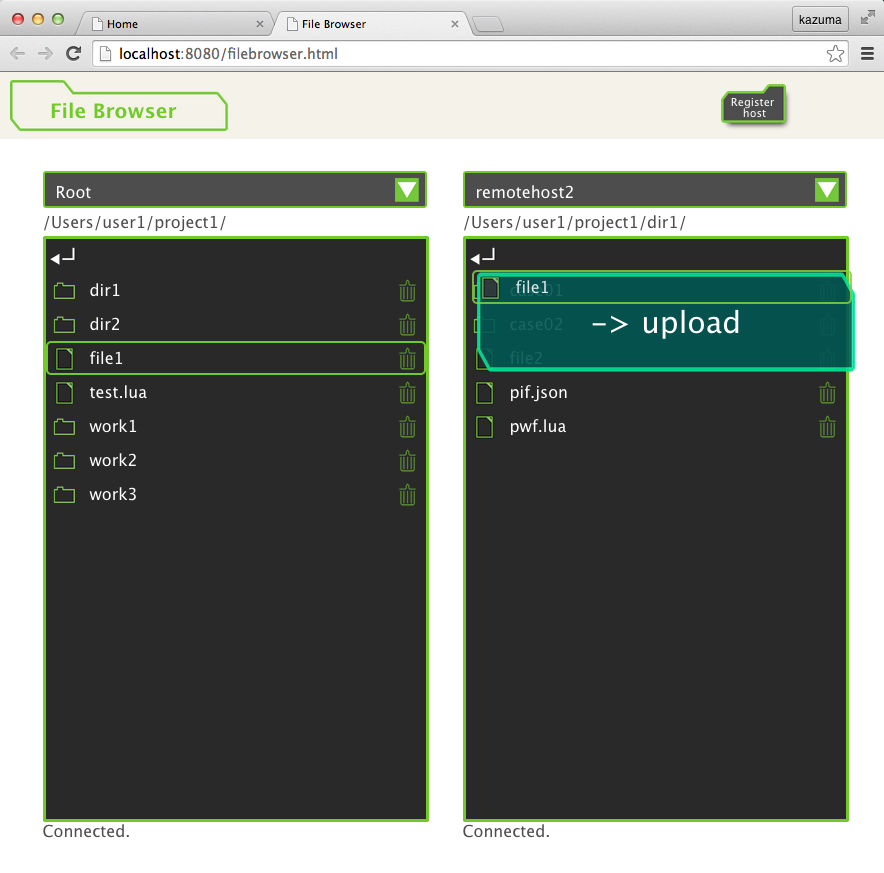
\includegraphics[width=12.0cm]{image/filebrowser_009.png}
	\end{center}
	\caption{ドラッグによるファイルのアップロード}
	\label{fig:filebrowser_fileupload}
\end{figure}

\newpage

\subsection{ファイルのダウンロード}
\begin{enumerate}
	\item 各ペインで,ダウンロード元(リモートホスト)とダウンロード先(ローカルホスト)のディレクトリを開きます.
	\item ダウンロードしたいファイルもしくはディレクトリをダウンロード元のペインからドラッグしてダウンロード先のペインに重ねると,
		  ファイル操作メニューが表示されます.
	\item 「download」上にドロップすることで,ドロップ先ディレクトリへのダウンロードが行われます.
\end{enumerate}

\begin{figure}[htbp]
	\begin{center}
		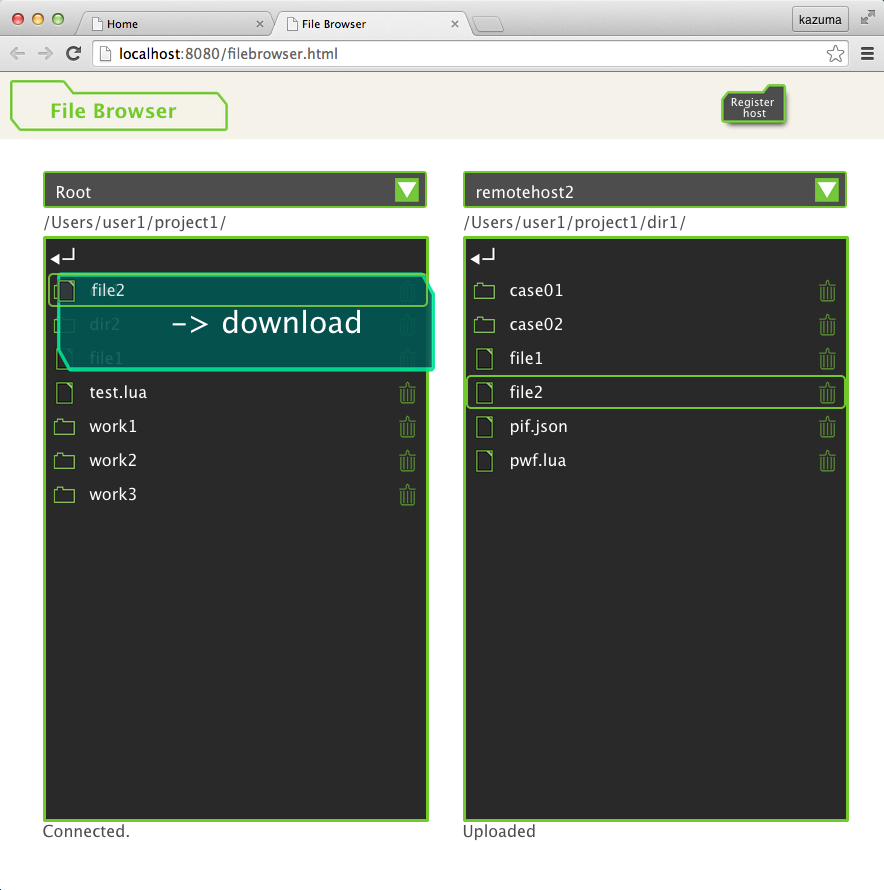
\includegraphics[width=12.0cm]{image/filebrowser_010.png}
	\end{center}
	\caption{ドラッグによるファイルのダウンロード}
	\label{fig:filebrowser_filedownload}
\end{figure}

\newpage

\chapter{プロジェクト編集画面}
\label{chap:projeditor}
プロジェクト編集画面では,プロジェクト情報の確認, プロジェクトディレクトリ内のファイルの閲覧,編集,ワークフロー実行制御およびコンソールによるログ確認を行います.

\begin{figure}[htbp]
	\begin{center}
		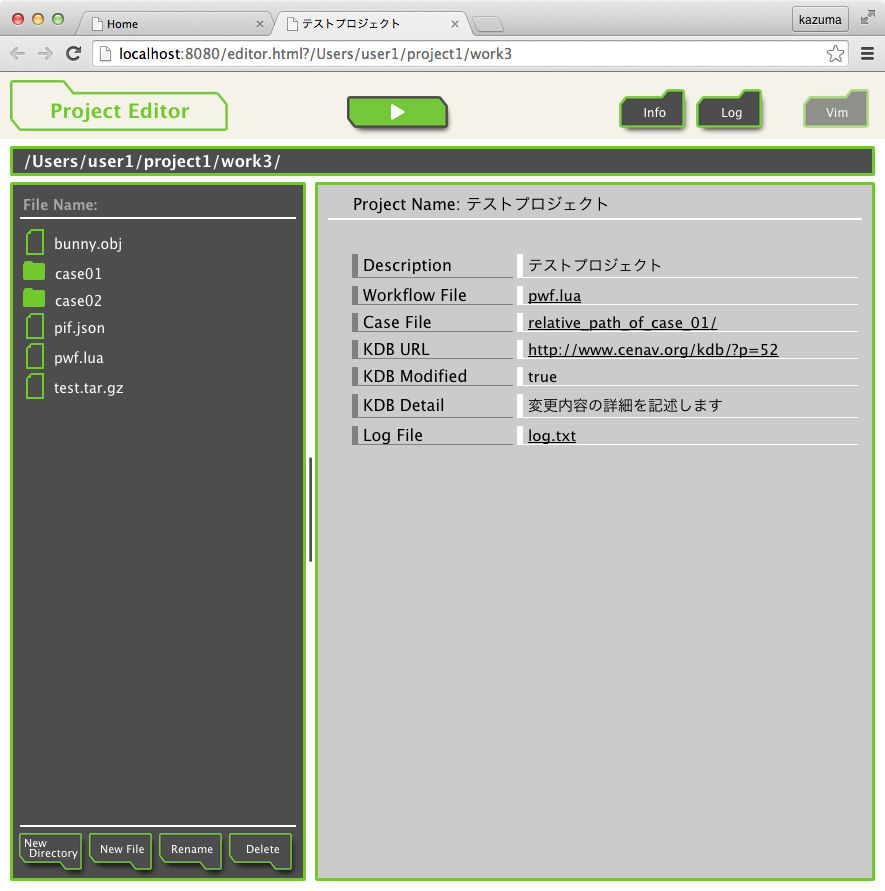
\includegraphics[width=12.0cm]{image/projeditor_000.png}
	\end{center}
	\caption{プロジェクト編集画面}
	\label{fig:projeditor}
\end{figure}

\newpage


\section{情報画面表示}
プロジェクト編集画面を新規に開くか, 「Info」ボタンを押すことで, 編集中のプロジェクト情報が表示されます(図\ref{fig:projeditor}). 
プロジェクト情報は, pif.jsonファイルによって定義された情報を元に表示しています.
また, 表示されたファイル名をクリックすることで, ファイルを閲覧することが出来ます.

\section{ディレクトリ移動とファイルの閲覧}
ファイル一覧からディレクトリを選択すると,そのディレクトリ内のファイル,ディレクトリがファイル一覧にツリー表示されます. また, テキスト形式のファイルを選択すると,それらのファイルの内容が右のペインに表示され,編集を行うことが出来ます.

\section{ファイルの新規作成}
「New File」ボタンを押すと,ファイル名入力ダイアログが表示されます.ファイル名を入力し,「New!」ボタンを押すと,現在開いているディレクトリ内に新規ファイルが作成されます.

\section{ディレクトリの新規作成}
「New Directory」ボタンを押すと,ディレクトリ名入力ダイアログが表示されます.ディレクトリ名を入力し,「New!」ボタンを押すと,現在開いているディレクトリ内に新規ディレクトリが作成されます.

\section{ファイル,ディレクトリ名の変更}
「Rename」ボタンを押すと, ファイル/ディレクトリ名入力ダイアログが表示されます. 名前を入力し, ポップアップ表示された「Rename」ボタンを押すと, 現在選択しているファイルまたはディレクトリ名が変更されます.

\section{ファイル,ディレクトリの削除}
ファイル/ディレクトリを選択した状態で, 「Delete」を押すと, 削除確認ダイアログが表示されます. ポップアップ表示された「Delete」ボタンを押すと, 現在選択しているファイルまたはディレクトリが削除されます.

\newpage

\section{ファイルの編集}
ファイル一覧からテキスト形式のファイルを選択すると,右のペインでファイルが開かれ,内容の編集が出来ます.

\begin{figure}[htbp]
	\begin{center}
		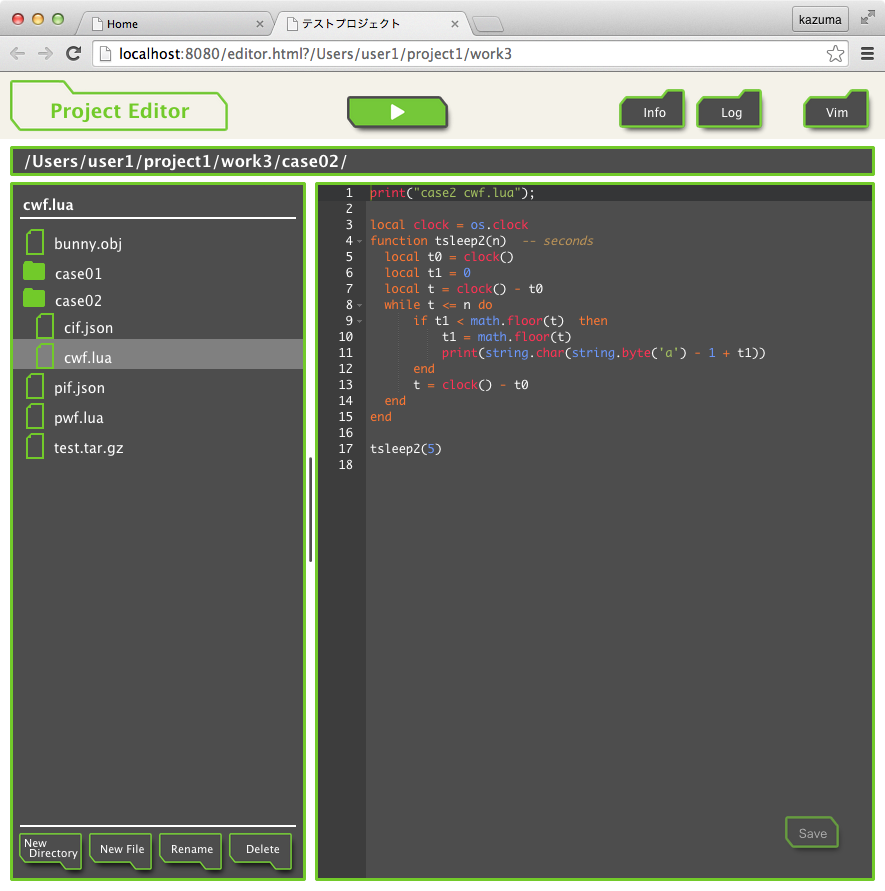
\includegraphics[width=12.0cm]{image/projeditor_003.png}
	\end{center}
	\caption{ファイルの編集}
	\label{fig:projeditor_edit}
\end{figure}

\newpage

\section{ファイルを開く}
\ref{sec:editconfig}にて"extension"に記述した拡張子のファイルをファイル一覧から選択すると,関連付けられたアプリケーションで開く,もしくはテキストとして右ペインのエディタ内で開くことが出来ます.

\begin{figure}[htbp]
	\begin{center}
		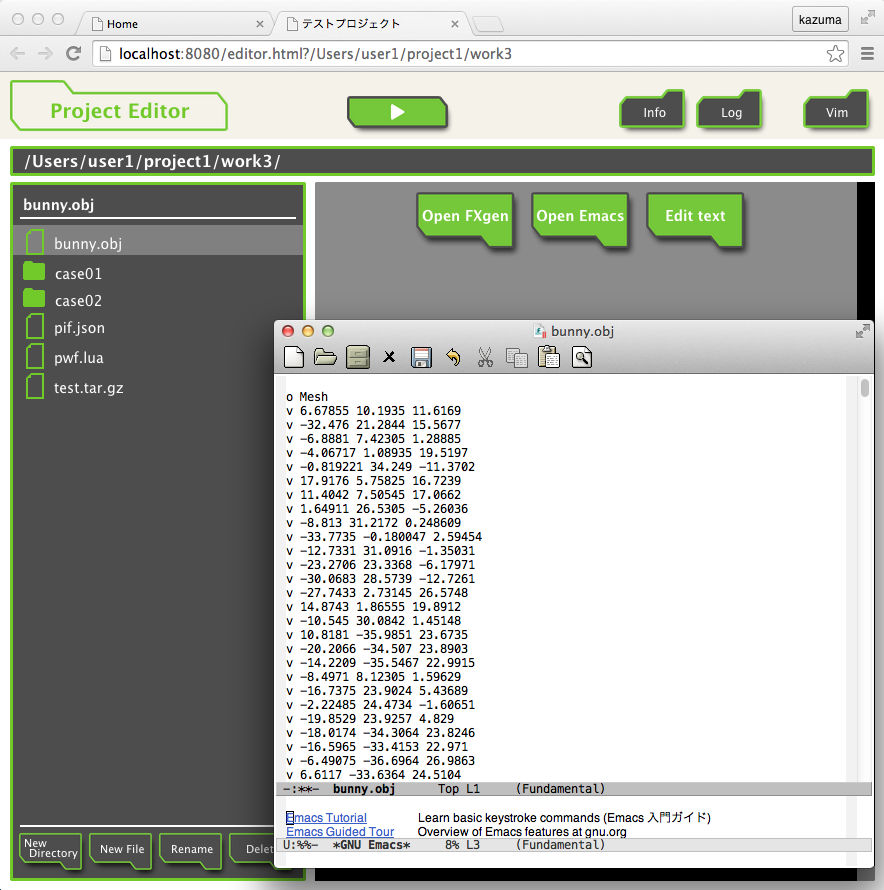
\includegraphics[width=12.0cm]{image/launch_button_003.png}
	\end{center}
	\caption{ファイルを開く}
	\label{fig:projeditor_edit}
\end{figure}

\section{ファイルの保存}
「SAVE」ボタンを押すと,右のペインで編集中のファイルが同名で上書き保存されます.

\section{ワークフローの実行}
プロジェクトエディタ上部のプロジェクト実行ボタンを押すと,ワークフローが実行されます. 実行中は, 実行ボタンが停止ボタンに切り替わります.

\begin{figure}[htbp]
	\begin{center}
		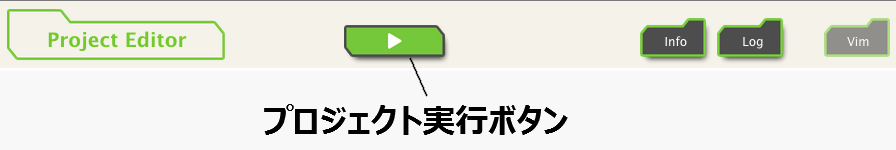
\includegraphics[width=12.0cm]{image/execute_project_button.png}
	\end{center}
	\caption{プロジェクト実行ボタン}
	\label{fig:execute_project_button}
\end{figure}

\section{ワークフローの停止}
ワークフローの実行中にプロジェクト停止ボタンを押すと,実行中のワークフローを停止出来ます.

\begin{figure}[htbp]
	\begin{center}
		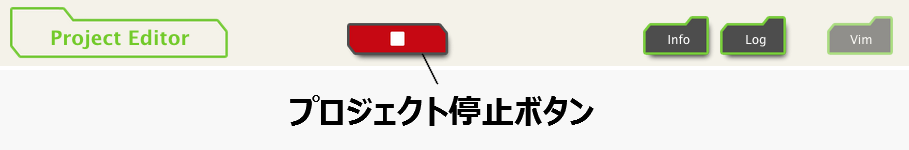
\includegraphics[width=12.0cm]{image/stop_project_button.png}
	\end{center}
	\caption{プロジェクト停止ボタン}
	\label{fig:stop_project_button}
\end{figure}

\section{コンソール(実行ログ)の表示}
「Log」ボタンを押すと,ポータルGUIの動作しているホスト上のコンソールが表示されます.

\begin{figure}[htbp]
	\begin{center}
		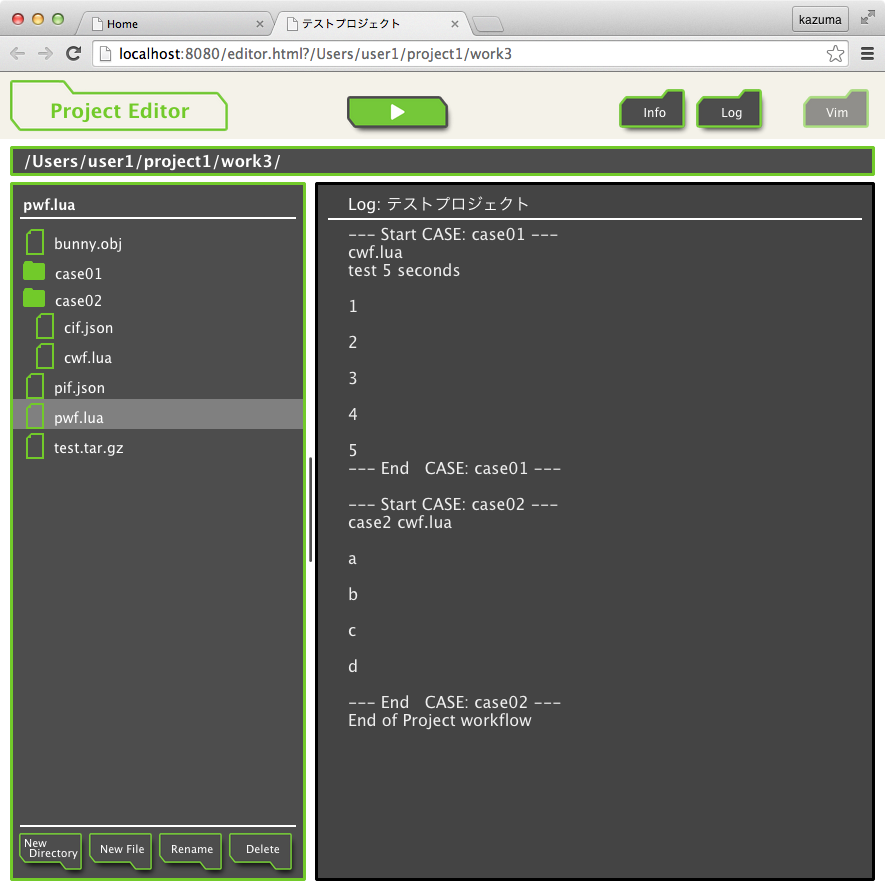
\includegraphics[width=12.0cm]{image/projeditor_004.png}
	\end{center}
	\caption{コンソールの表示}
	\label{fig:projeditor_comsole}
\end{figure}

\section{エディットモードの切り替え}
「Vim」/「Default」ボタンで,エディタ部分のキーボードバインドが変更出来ます.

\end{document}

